%
%%%%%
%%%%%

\documentclass[mathserif,graphics]{beamer}
\usepackage{Sweave}
\usepackage[labelformat=empty]{caption}
\mode<presentation>
\usetheme{Frankfurt} % Beamer Theme
\setbeamersize{text margin left=5mm, text margin right=5mm}
\usecolortheme{whale}
\usepackage{amsmath} % for math AMS fonts
\usepackage{centernot}
\usepackage{graphicx} % to include figures
\usepackage{subfigure} % to have figures in figures
\usepackage{multimedia} % to include movies

\usepackage[utf8]{inputenc}
\usepackage{amsfonts}
\usepackage{natbib}
\usepackage{scrpage2}
\usepackage{dsfont}
\usepackage{float}
\usepackage{amssymb}

\usepackage{bbm}

\usepackage{tikz}
\usepackage{colortbl}
\usepackage{mdframed}
\usepackage{boxedminipage}
\usetikzlibrary{arrows,shapes,backgrounds, patterns, decorations.markings} % loads some tikz extensions
\usepackage[english]{babel}
\useoutertheme[subsection=false]{smoothbars} % Beamer Outer Theme
\usepackage{mdframed}
\usepackage{boxedminipage}
\newcommand{\hlcolor}[2]{{\setlength{\fboxsep}{0pt}\colorbox{#1}{\strut #2}}}
\newcommand{\eg}{e.\,g. }
\newcommand{\ie}{i.\,e. }
\newcommand{\cdf}{c.\,d.\,f. }
%\usepackage[usenames,dvipsnames]{xcolor}
\definecolor{lightblue}{rgb}{0.8,0.85,1}

\newcommand{\bi}{\begin{itemize}}
\newcommand{\ei}{\end{itemize}}
\newcommand{\be}{\begin{enumerate}}
\newcommand{\ee}{\end{enumerate}}

\newcommand{\hl}[1]{\textcolor{red}{#1}}

\defbeamertemplate*{footline}{my infolines theme}
    {
      \leavevmode%
      \hbox{%
      \begin{beamercolorbox}[wd=.44\paperwidth,ht=2.25ex,dp=1ex,center]{author
      in head/foot}%
        \usebeamerfont{author in head/foot}\insertshortauthor~~\insertshortinstitute
      \end{beamercolorbox}%
      \begin{beamercolorbox}[wd=.2\paperwidth,ht=2.25ex,dp=1ex,center]{title in
      head/foot}%
        \usebeamerfont{title in head/foot}\insertshorttitle
      \end{beamercolorbox}%
      \begin{beamercolorbox}[wd=.36\paperwidth,ht=2.25ex,dp=1ex,right]{date in
      head/foot}%
        \usebeamerfont{date in head/foot}\insertshortdate{}\hspace*{2em}
        \insertframenumber{} / \inserttotalframenumber\hspace*{2ex}
      \end{beamercolorbox}}%
      \vskip0pt%
    }

\title{Normal Distribution}
%\subtitle{Seminar graph algorithms}
\author{Andrey Chinnov, Sebastian Honermann, Carlos Zydorek}
%\institute{Seminar graph algorithms}
\date{Case Studies \\
"Data Analytics"}

\begin{document}
\frame{
\titlepage
\setbeamercovered{dynamic}
}

\begin{frame}
\frametitle{Outline}
\tableofcontents
\end{frame}


\section{Introduction}

\subsection{Normality as a requirement for statistical methods}

\subsection{Normality as a requirement for statistical methods}

\frame{
\frametitle{Normality as a requirement for statistical methods}
Many statistical tests assume data to be drawn from a normal distribution
\bi
\item Two-sample z-test
\item One-sample t-test
\item Chi-squared test for variance \dots
\ei

\begin{block}{Density function of the univariate normal distribution}
\[ Pr(x) = \frac{1}{\sqrt{2\pi\sigma^2}}\,\mbox{exp}\left\{-\frac{1}{2\sigma^2}(x - \mu)^2\right\} \]
with the parameters mean $\mu \in \mathbb{R}$ and variance $\sigma > 0$
\end{block}

\begin{block}{Density function of the multivariate normal distribution}
\[Pr(x) = |2\pi\Sigma|^{-1/2} \,\mbox{exp}\left\{-\frac{1}{2}(x-\mu)' \Sigma^{-1}(x-\mu)\right\}\]
with mean vector $\mu$ and covariance $\Sigma$ > 0
\end{block}
}

\subsection{Data Set Overview}

\frame{
\frametitle{Data Set Overview}
\bi\setlength\parskip{8pt}
\item \texttt{Glass} data set from package \texttt{mlbench}
\item sample of 214 observations
\item 7 \hl{types} of glass (but only 6 present in this sample)
\item \hl{Variables:} refractive index (RI) and 8 elements (Na, Mg, Al, Si, K, Ca, Ba, Fe)
\ei
}

\section{Transformation to Normality}
\subsection{}
\frame{
\frametitle{Box-Cox Transformation}
\framesubtitle{Definition}
\begin{block}{Box-Cox Transformation}
If data are not normally distributed, they can possibly be transformed by the parameterised power transformation
\[
  \phantom{\quad\mbox{for}\ x > 0}
   x^{(\lambda)} =
   \left\{ 
    \begin{array}{cl}
%\vspace{12pt}
                 \frac{x^\lambda - 1}{\lambda} & \lambda \neq 0\\
                 \ln(x) & \lambda = 0
    \end{array}
   \right.
   \quad\mbox{for}\ x > 0
\]
\end{block}

The optimal parameter $\lambda$ for specific observations $x_1, \dots, x_n$ can be obtained by a \hl{maximum-likelihood} estimation, maximising the log likelihood
\[
\begin{array}{l}
\vspace{12pt}
   l(\lambda) = - \frac{n}{2}\ln\left[\frac{1}{n}\sum_{j=1}^{n}(x_j^{(\lambda)} - \overline{x^{(\lambda)}})^2\right] + (\lambda - 1) \sum_{j=1}^{n}\ln(x_j)\\
   \mbox{with}\ \overline{x^{(\lambda)}} = \frac{1}{n} \sum_{j=1}^{n}x_j^{(\lambda)}
\end{array}
\]
}

\frame{
\frametitle{Box-Cox Transformation}
\framesubtitle{Transformation issues}
\begin{center}
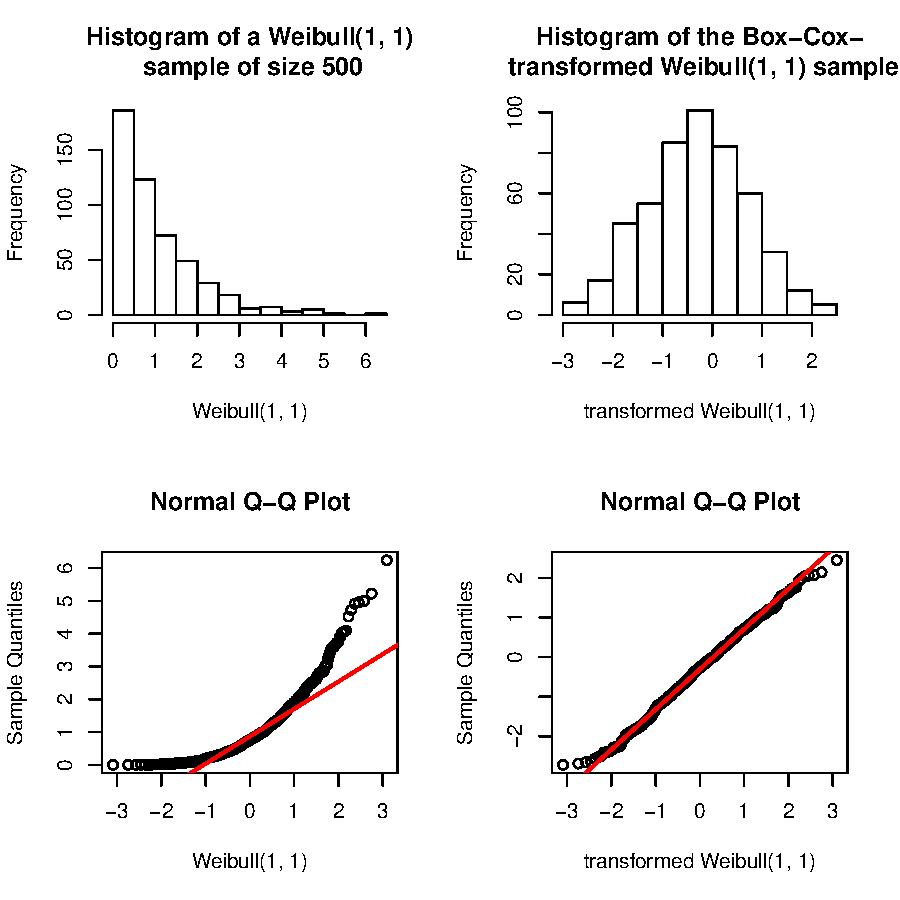
\includegraphics[width=0.6\textwidth]{report-transformationUnimodal}
\end{center}
}

\frame{
\frametitle{Box-Cox Transformation}
\framesubtitle{Transformation issues}
\begin{center}
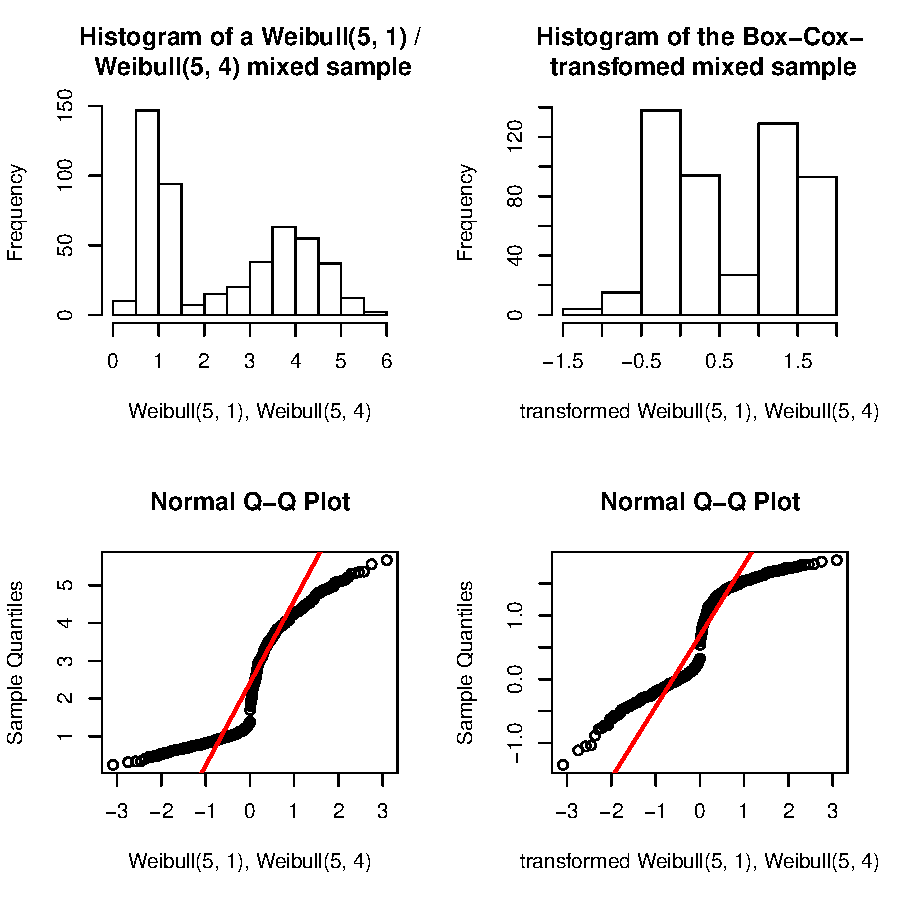
\includegraphics[width=0.6\textwidth]{report-transformationBimodal}
\end{center}
}

\section{Normality Testing}

\subsection{Univariate case}

\frame{
\frametitle{Q-Q-Plots}
\footnotesize
\begin{columns}[t]
\column{0.3\columnwidth}
{\bf Sample:}
\[x=(x_1,x_2,\dots,x_n)\]
{\bf Empirical quantiles:}
\[x_{(1)}\le x_{(2)} \le \dots \le x_{(n)}\]
{\bf Theoretical quantiles:}
\[q_{(j)} = \Phi^{-1}(p_{(j)}),\]
where
\[ p_{(j)} = \frac{j - \frac{1}{2}} {n},\]
\[\Phi\mbox{ - }N(0,1)\mbox{ \cdf.}\]

\[\implies \mbox{ Plot } x_{(i)}\mbox{ against } q_{(i)}\]
\vspace{15cm}
\column{0.7\columnwidth}
\vspace{-1.35cm}
\begin{figure}
	\includegraphics[width=\columnwidth]{report-QQfull}
	\end{figure}
\end{columns}
\vspace{15cm}
}

\frame{
\frametitle{Q-Q-Plots}
\footnotesize
\begin{columns}[t]
\column{0.4\columnwidth}
\centerline{{\bf QQ-Plots of the subdatasets:}}

\begin{itemize}
\item Variables could be normally distributed within the subclasses 
\item For some cases there appear to be a linear relationships
\item For other cases a linear relationship is questionable
\item In some subdatasets a linear relationship seems plausible, however $n$ is very small
\end{itemize}
\vspace{15cm}
\column{0.6\columnwidth}
\vspace{-1cm}
\begin{figure}
	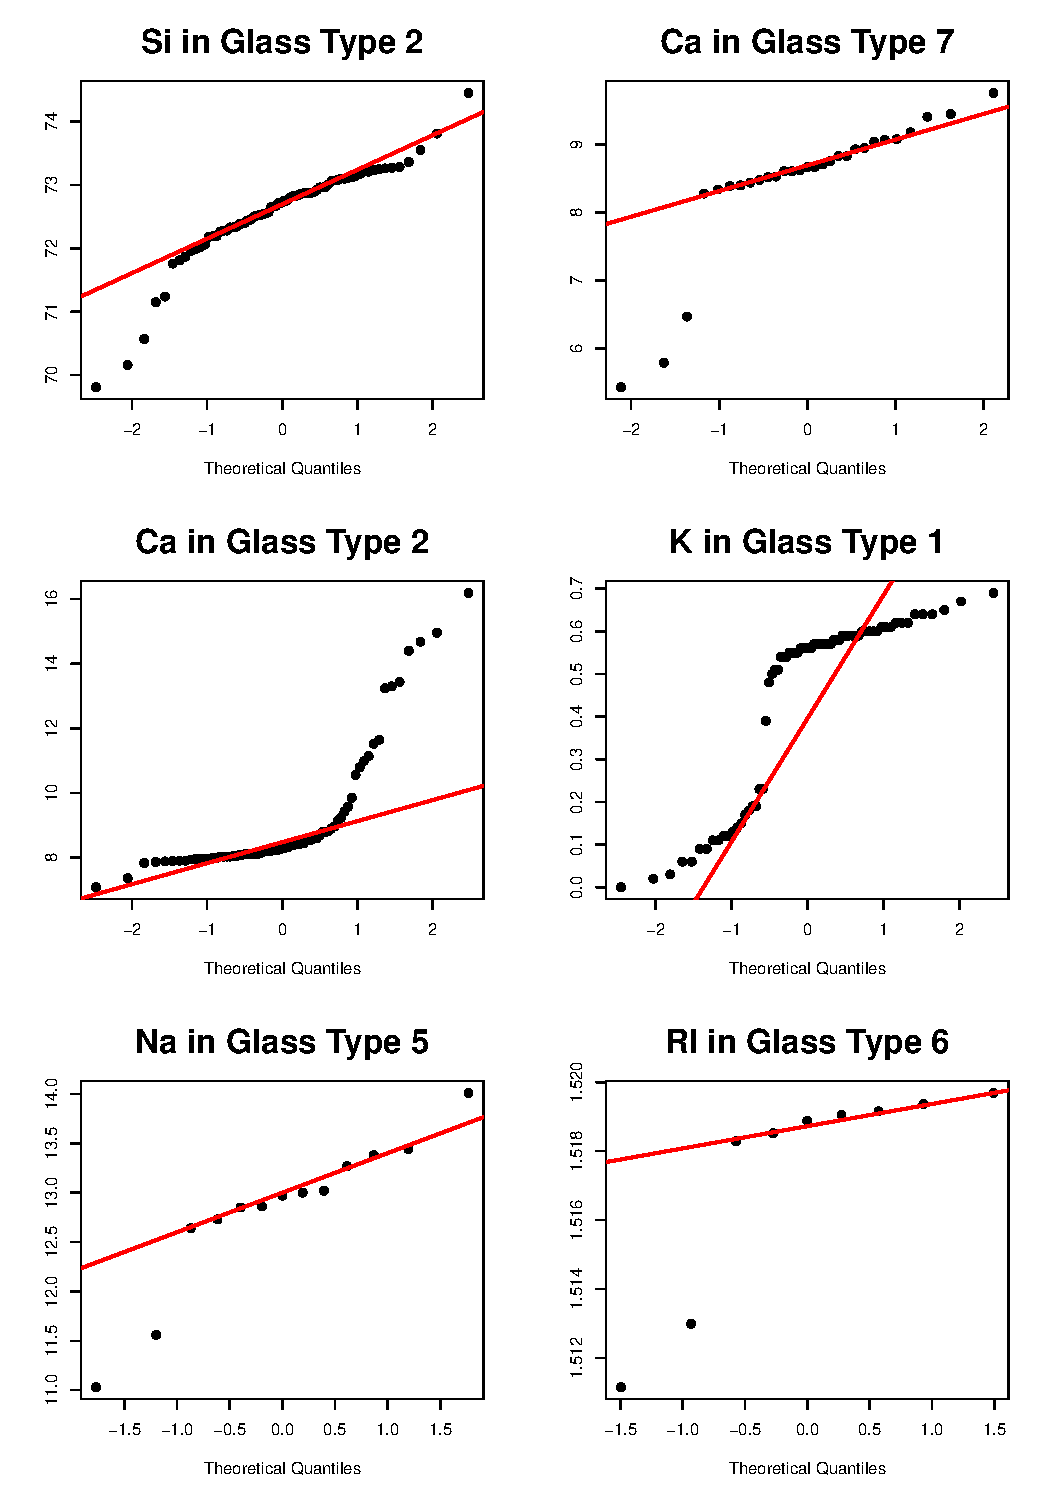
\includegraphics[width=0.8\columnwidth]{graph}
	\end{figure}
\end{columns}
\vspace{15cm}
}

\frame{
\frametitle{Q-Q-Plots}
\footnotesize
\begin{columns}[t]
\column{0.4\columnwidth}
\begin{center}
{\bf Results of the Transformation of the Full Dataset
:}
\end{center}

\begin{itemize}
\item For some of the cases there seems to be a slight improvement

\item For non-unimodal cases the transformation does not show significant improvements towards normality
\end{itemize}
\vspace{15cm}
\column{0.6\columnwidth}
\vspace{-1cm}
\begin{figure}
	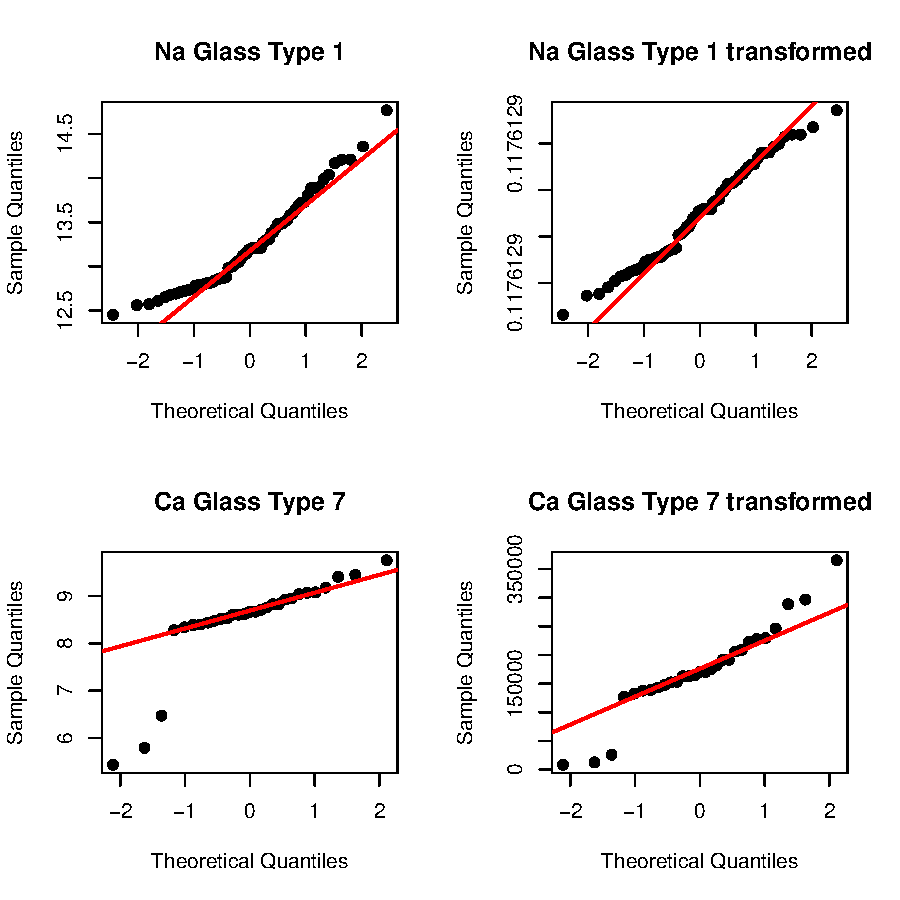
\includegraphics[width=\columnwidth]{Report-QQtrans}
	\end{figure}
\end{columns}
\vspace{15cm}
}

\frame{
\frametitle{Q-Q-Plots}
\footnotesize
\begin{columns}[t]
\column{0.4\columnwidth}
\begin{center}
{\bf Results of the Transformation of the Subdatasets
:}
\end{center}

\begin{itemize}
\item For unimodal cases the transformation shapes the distribution closer to normality

\item For non-unimodal cases the transformation does not show significant improvements towards normality
\end{itemize}
\vspace{15cm}
\column{0.6\columnwidth}
\vspace{-1cm}
\begin{figure}
	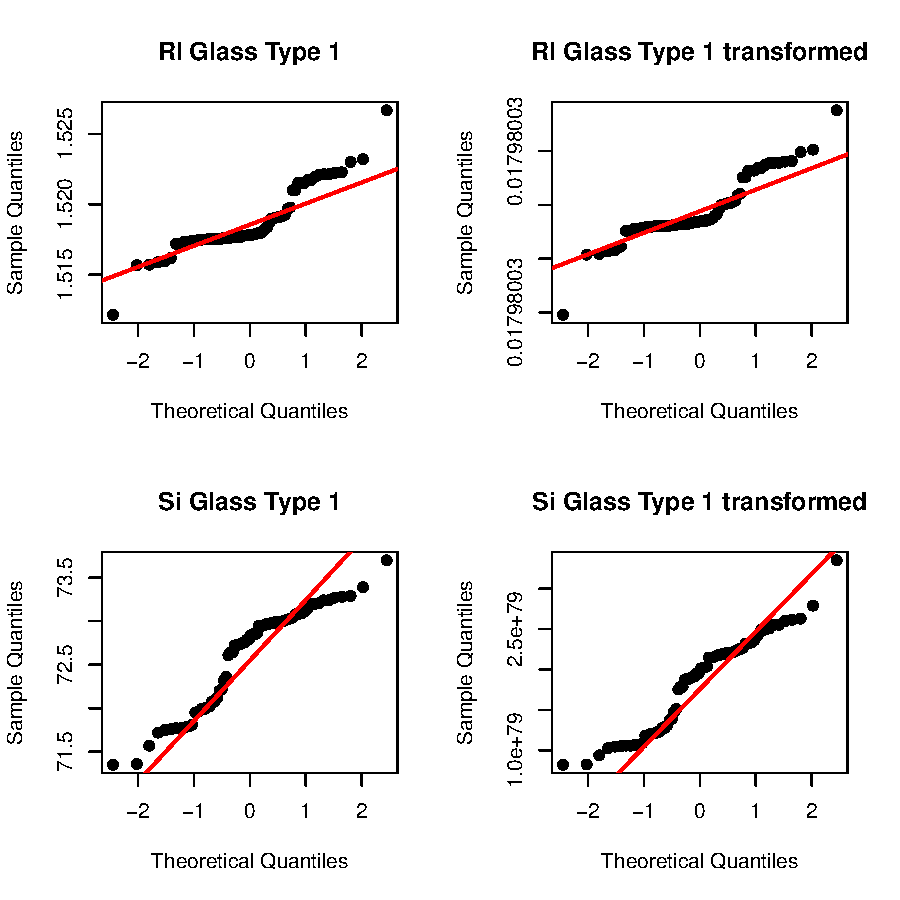
\includegraphics[width=\columnwidth]{Report-QQtransno}
	\end{figure}
\end{columns}
\vspace{15cm}
}

\frame{
\frametitle{Shapiro-Wilk Test}
The test statistic $W$ indicates the deviation of the observed quantile values from the assumed cumulative distribution function quantiles 
\[W = \frac{\sum  \limits_{i=1}^n(a_i y_i)^2}{\sum  \limits_{i=1}^n (y_i-\bar{y})^2},\]
where
\begin{itemize}
\item $a_i$ denotes the normalised "best linear unbiased" coefficients,
\item $y_i$ denotes the observations.
\end{itemize}

The critical value for $W$ is obtained by the Monte Carlo Method\\
$\implies$ $p$-value is calculated

\alert{Important:} If a variable contains only zeros the Shapiro-Wilk test is not applicable, 
since the term in the denominator sums up to zero.
}

\frame{
\frametitle{Shapiro-Wilk Test}
\begin{columns}[t]
\column{0.23\columnwidth}
\scriptsize
\vspace{-0.5cm}
\begin{center}
{\bf Testing the Full Dataset
:}
\end{center}
Null hypothesis is rejected for all variables at a 1 \% significance level
\begin{center}
{\bf After the Transformation
:}
\end{center}

The null hypothesis can be rejected for the four transformed variables

\alert{$\implies$ Possible Explanation:} Combination of different 	
distributions in the different glass types
\vspace{15cm}
\column{0.77\columnwidth}
\tiny
\vspace{-0.8cm}
\begin{table}[h!]
\centering
\begin{tabular}{|cccccc|} \hline variable & test statistic & sig. level & critical value & p-value & rejected\\ \hline RI & 0.87 & 0.01 & NA & 1.0766713449726e-12 & yes\\ 
Na & 0.95 & 0.01 & NA & 3.4655430546966e-07 & yes\\ 
Mg & 0.7 & 0.01 & NA & < 1.0e-15 & yes\\ 
Al & 0.94 & 0.01 & NA & 2.08315629600399e-07 & yes\\ 
Si & 0.92 & 0.01 & NA & 2.17503176825416e-09 & yes\\ 
K & 0.44 & 0.01 & NA & < 1.0e-15 & yes\\ 
Ca & 0.79 & 0.01 & NA & < 1.0e-15 & yes\\ 
Ba & 0.41 & 0.01 & NA & < 1.0e-15 & yes\\ 
Fe & 0.65 & 0.01 & NA & < 1.0e-15 & yes\\ \hline \end{tabular}
\caption{\scriptsize Test results of the Shapiro-Wilk test on the whole
data sample}
\end{table}
\vspace{-1cm}
\begin{table}[h!]
\centering
\begin{tabular}{|cccccc|} \hline variable & test statistic & sig. level & critical value & p-value & rejected\\ \hline RI & NA & NA & NA & NA & NA\\ 
Na & 0.95 & 0.01 & NA & 8.75605777309153e-07 & yes\\ 
Mg & NA & NA & NA & NA & NA\\ 
Al & 0.97 & 0.01 & NA & 0.000244326513056066 & yes\\ 
Si & 0.93 & 0.01 & NA & 1.58998125691823e-08 & yes\\ 
K & NA & NA & NA & NA & NA\\ 
Ca & 0.89 & 0.01 & NA & 1.13880689831982e-11 & yes\\ 
Ba & NA & NA & NA & NA & NA\\ 
Fe & NA & NA & NA & NA & NA\\ \hline \end{tabular}
\caption{\scriptsize Test results of the Shapiro-Wilk test on the whole
transformed data sample}
\end{table}
\vspace{15cm}
\end{columns}
}

\frame{
\frametitle{Shapiro-Wilk Test}
\begin{columns}[t]
\column{0.23\columnwidth}
\scriptsize
\vspace{-0.5cm}

{\bf Testing the Subdatasets Example – Glass Type 1
:}\\
\vspace{0.25cm}
Null hypothesis is rejected for all variables at a 1 \% significance level\\
\vspace{0.5cm}

{\bf After the Transformation
:}\\
\vspace{0.25cm}
The null hypothesis cannot be rejected for 3 of the transformed variables\\
\vspace{0.3cm}
\alert{$\implies$} 
Appearently the 	transformation was 	successful
\vspace{15cm}
\column{0.77\columnwidth}
\tiny
\vspace{-0.8cm}
\begin{table}[h!]
\centering
\begin{tabular}{|cccccc|} \hline variable & test statistic & sig. level & critical value & p-value & rejected\\ \hline RI & 0.88 & 0.01 & NA & 6.36192013015468e-06 & yes\\ 
Na & 0.95 & 0.01 & NA & 0.00459078607995831 & yes\\ 
Mg & 0.82 & 0.01 & NA & 8.02702432879544e-08 & yes\\ 
Al & 0.9 & 0.01 & NA & 5.42971629496434e-05 & yes\\ 
Si & 0.91 & 0.01 & NA & 0.000117060780025464 & yes\\ 
K & 0.77 & 0.01 & NA & 3.14049093233846e-09 & yes\\ 
Ca & 0.93 & 0.01 & NA & 0.00103561283726753 & yes\\ \hline \end{tabular}
\caption{\scriptsize Test results of the Shapiro-Wilk test on type 1 glass}
\end{table}
\begin{table}[h!]
\centering
\begin{tabular}{|cccccc|} \hline variable & test statistic & sig. level & critical value & p-value & rejected\\ \hline RI & 0.89 & 0.01 & NA & 1.62433657125306e-05 & yes\\ 
Na & 0.98 & 0.01 & NA & 0.353792914291578 & no\\ 
Mg & 0.83 & 0.01 & NA & 1.40023833110547e-07 & yes\\ 
Al & 0.96 & 0.01 & NA & 0.0459207068393172 & no\\ 
Si & 0.94 & 0.01 & NA & 0.00269629206710463 & yes\\ 
K & NA & NA & NA & NA & NA\\ 
Ca & 0.97 & 0.01 & NA & 0.148237775100495 & no\\ \hline \end{tabular}
\caption{\scriptsize Test results of the Shapiro-Wilk test on the transformed
type 1 glass}
\end{table}
\vspace{15cm}
\end{columns}
}

\frame{
\frametitle{Pearson's Chi-Squared Test}
\framesubtitle{Theoretical foundations}

\bi
\item Divide observations $X_1, \dots, X_N$ into \hl{pairwise disjoint classes} $C_1, \dots, C_K$
\item Common requirement: minimum class size of 5
\item Compare \hl{observed} class frequencies to \hl{expected} theoretical class frequencies for a certain distribution
\ei
\[\mbox{test statistic:}\quad\chi^2 = \sum_{k=1}^{K}\frac{(O_k - E_k)^2}{E_k}\]
\bi
\item The test statistic is approximately \hl{$\chi^2$-distributed} with $K-1$ degrees of freedom (minus one degree of freedom per estimated parameter)
\ei
}

\begin{frame}<1>[label=zoom]
\frametitle{Pearson's Chi-Squared Test}
\framesubtitle{Theoretical foundations}
\framezoom<1><2>(7.8cm, 2.65cm)(3.7cm, 2.9cm)
\vspace{50pt}

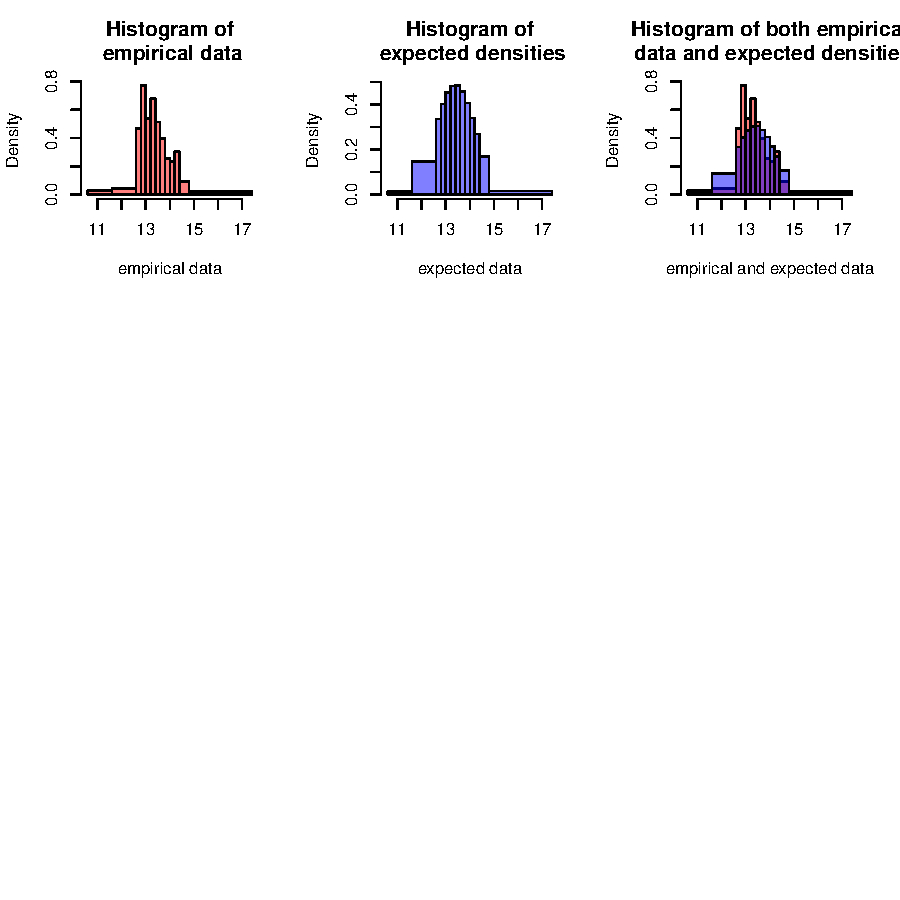
\includegraphics[width=\textwidth]{presentation-chisqSampleHist}
\end{frame}

\frame{
\frametitle{Pearson's Chi-Squared Test}
\framesubtitle{Theoretical foundations}

\bi
\item Test under the \hl{null hypothesis} that the sample is drawn from a population with unknown distribution $\mathbb{P}$ which is equal to the assumed distribution $\mathbb{P}_0$:
\[\begin{array}{rcl}
H_0 & : & \mathbb{P} = \mathbb{P}_0,\\
H_1 & : & \mathbb{P} \neq \mathbb{P}_0.
\end{array}\]
\ei
\begin{block}{Decision rule}
\[
  %\phantom{\quad\mbox{with}\ F=\chi^2_{K-1-p}}
  \delta =
   \left\{ 
    \begin{array}{cll}
%\vspace{12pt}
                 1 & \mbox{if} \ \chi^2 > F^{-1}(1-\alpha)\\
                 0 & \mbox{otherwise}
    \end{array} 
   \right.
   \quad\mbox{with}\ F=\chi^2_{K-1-p}
\]
\[(\mbox{significance level}\ \alpha,\quad \mbox{number of estimated parameters}\ p)\]
\end{block}
}

\frame{
\frametitle{Pearson's Chi-Squared Test}
\framesubtitle{Test results for the whole sample}
\scriptsize
\begin{center}
\begin{tabular}{|cccccc|} \hline variable & test statistic & sig. level & critical value & p-value & rejected\\ \hline RI & 64.95 & 0.01 & 13.28 & 2.64011035255862e-13 & yes\\ 
Na & 36.99 & 0.01 & 13.28 & 1.80797974702607e-07 & yes\\ 
Mg & 158.3 & 0.01 & 11.34 & < 1.0e-15 & yes\\ 
Al & 27.2 & 0.01 & 9.21 & 1.24084046404516e-06 & yes\\ 
Si & 38.85 & 0.01 & 13.28 & 7.4876188027595e-08 & yes\\ 
K & 95.97 & 0.01 & NA & NA & NA\\ 
Ca & 131.13 & 0.01 & 13.28 & < 1.0e-15 & yes\\ 
Ba & 31.37 & 0.01 & NA & NA & NA\\ 
Fe & 70.96 & 0.01 & 13.28 & 1.4210854715202e-14 & yes\\ \hline \end{tabular}
\end{center}
}

\frame{
\frametitle{Pearson's Chi-Squared Test}
\framesubtitle{Test results for type 1 glass}
\scriptsize
\begin{center}
\begin{tabular}{|cccccc|} \hline variable & test statistic & sig. level & critical value & p-value & rejected\\ \hline RI & 28.01 & 0.01 & 9.21 & 8.26265138420545e-07 & yes\\ 
\alt<2>{\cellcolor{yellow}Na}{Na} & \alt<2>{\cellcolor{yellow}3.25}{3.25} & \alt<2>{\cellcolor{yellow}0.01}{0.01} & \alt<2>{\cellcolor{yellow}13.28}{13.28} & \alt<2>{\cellcolor{yellow}0.51688441877949}{0.51688441877949} & \alt<2>{\cellcolor{yellow}no}{no}\\ 
Mg & 18.81 & 0.01 & 6.63 & 1.44068580684165e-05 & yes\\ 
Al & 23.55 & 0.01 & 11.34 & 3.10284613768141e-05 & yes\\ 
Si & 23.68 & 0.01 & 13.28 & 9.26014020323773e-05 & yes\\ 
K & 114.86 & 0.01 & 11.34 & < 1.0e-15 & yes\\ 
Ca & 22.58 & 0.01 & 15.09 & 0.000405198755082603 & yes\\ 
Fe & 18.65 & 0.01 & 9.21 & 8.91413549507503e-05 & yes\\ \hline \end{tabular}
\end{center}
}

\frame{
\frametitle{Pearson's Chi-Squared Test}
\framesubtitle{Test results for sodium of type 1 glass}
\scriptsize
\begin{center}

\begin{minipage}{0.49\textwidth}
\begin{tabular}{|c|cc|} \hline class & \multicolumn{2}{c|}{frequencies}\\ (interval) & observed & expected\\ \hline ]12.4, 12.8] & 15 & 13.15\\ 
]12.8, 13] & 12 & 8.81\\ 
]13, 13.2] & 9 & 10.68\\ 
]13.2, 13.4] & 11 & 11.04\\ 
]13.4, 13.6] & 8 & 9.74\\ 
]13.6, 14] & 9 & 12.06\\ 
]14, 14.8] & 6 & 4.52\\ \hline \end{tabular}
\end{minipage}
\hfill
\begin{minipage}{0.49\textwidth}
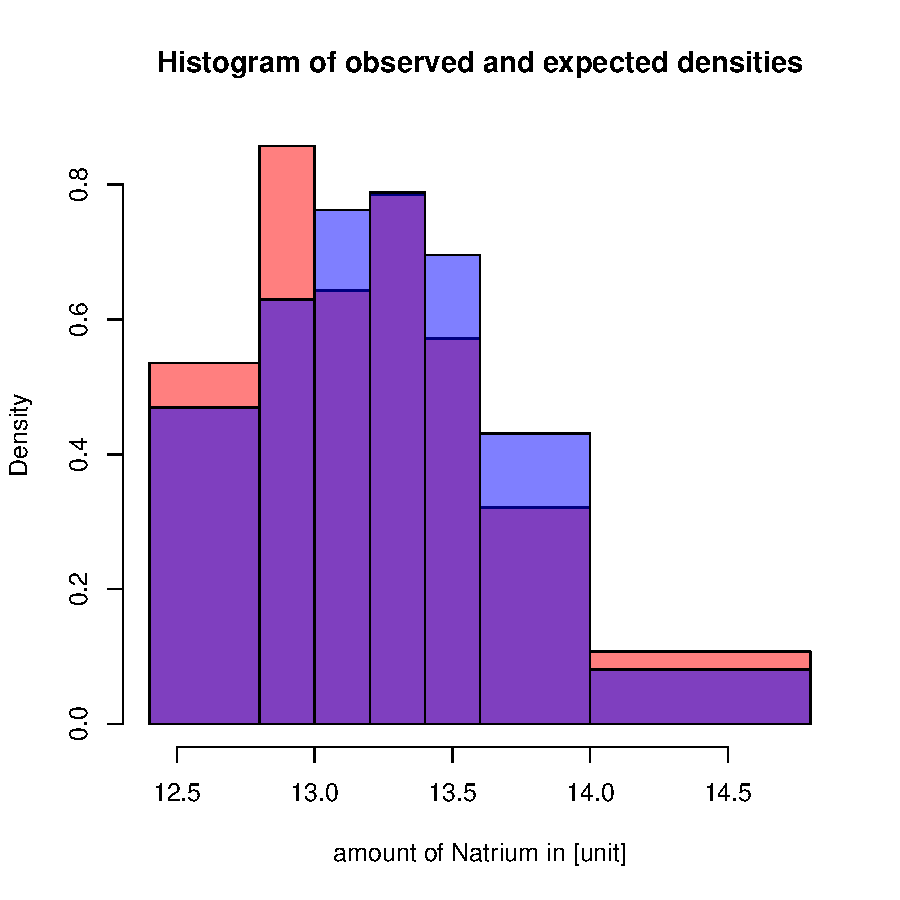
\includegraphics[width=0.8\textwidth]{report-chisqType1Na}
\end{minipage}
\end{center}
}

\frame{
\frametitle{Pearson's Chi-Squared Test}
\framesubtitle{Test results for transformed type 1 glass}
\scriptsize
\begin{center}
\begin{tabular}{|cccccc|} \hline variable & test statistic & sig. level & critical value & p-value & rejected\\ \hline RI & 27.81 & 0.01 & 6.63 & 1.33864150764218e-07 & yes\\ 
Na & 1.59 & 0.01 & 13.28 & 0.810360513797024 & no\\ 
Mg & 17.87 & 0.01 & NA & NA & NA\\ 
Al & 6.41 & 0.01 & 11.34 & 0.093110657016404 & no\\ 
Si & 16.87 & 0.01 & 13.28 & 0.00205136639513992 & yes\\ 
K & NA & 0.01 & NA & NA & NA\\ 
Ca & 3.35 & 0.01 & 11.34 & 0.341234021909645 & no\\ 
Fe & NA & 0.01 & NA & NA & NA\\ \hline \end{tabular}
\end{center}
}

\frame{
\frametitle{Kolmogorov-Smirnov Test}
\framesubtitle{Preliminaries}
Let $x=(x_1,x_2, \dots, x_n)$ be a sample of unknown
distribution $\mathbb{P}$.
\begin{columns}[t]
\column{0.5\columnwidth}
\vspace{-0.5cm}
\begin{definition}
$F_n(x)=\frac{1}{n}\sum_{i=1}^n \mathbbm{1}_{\{x_i\le x\}}(x)$ \\
- \alert{empirical} \cdf, where \\
$\mathbbm{1}_{\{x_i\le x\}}(x)=\left\lbrace 
\begin{array}{cll}
                1 & \mbox{if} \ x_i\le x\\
                 0 & \mbox{otherwise}.
\end{array} 
\right.$
\end{definition}
\onslide<2->{
$F(x)$ - theoretical normal \cdf with
\[\bar{x}=\frac{1}{n}\sum_i x_i,\quad \sigma^2_x=\frac{1}{n}(x_i-\bar{x})^2\]}
\onslide<3->{
$d=\sup_{x\in \mathbb{R}}|F_n(x)-F(x)|$ \\- distance between them.}
\column{0.5\columnwidth}
  \vspace{-1cm}
    \only<1>{
    \begin{figure}
	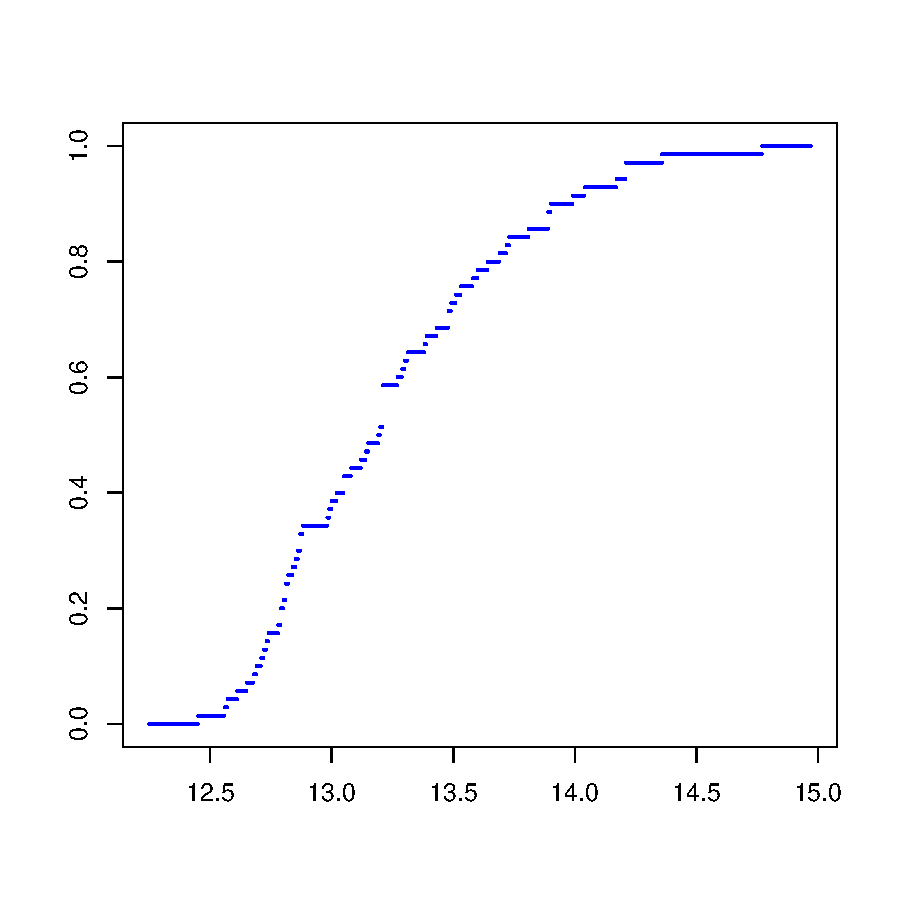
\includegraphics[width=\columnwidth]{Report-empiricFunc}
	\end{figure}}
    \only<2->{
    \begin{figure}
	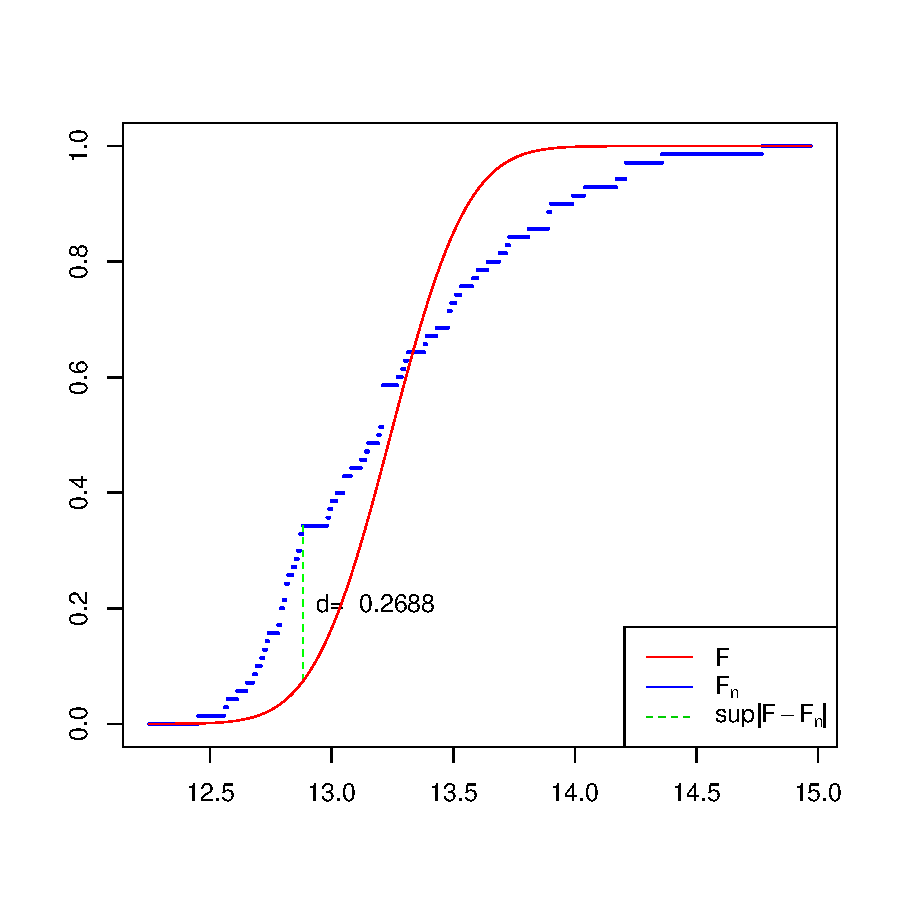
\includegraphics[width=\columnwidth]{Report-empiricTeorFunc}
	\end{figure}}
\vspace{-1.5cm}
\begin{center}
Glass Type 1, Sodium (Na)
\end{center}
\end{columns}
}

\frame{
\frametitle{Kolmogorov-Smirnov Test}
Let $x=(x_1,x_2, \dots, x_n)$ be a sample of unknown
distribution $\mathbb{P}$.\\
Theoretical \cdf $F$ defines a distribution $\mathbb{P}_0$.\\
\onslide<2->{
\[\begin{array}{rcl}
H_0 & : & \mathbb{P} = \mathbb{P}_0,\\
H_1 & : & \mathbb{P} \ne \mathbb{P}_0.
\end{array}\]}
\onslide<3->{
KS test statistics:
\[D_n = \sqrt{n}\cdot \sup_{x \in \mathbb{R}}|F_n(x)-F(x)|.\]}
\onslide<4->{
Properties of $D_n$ in case $H_0$ is \alert{TRUE}:}
\begin{itemize}
\item<4-> Distribution of $\hat{D}_n:=(D_1,D_2,\dots, D_n)$ does not depend on
$F$\\
\onslide<5->{\hfill$\implies$ \alert{tabulated}}
\item<6-> $\forall t>0:$ \[P(D_n\le t)\xrightarrow[n \to \infty]{}
H(t)=1-2\sum_{i=1}^{\infty}(-1)^{i-1} \exp^{-2i^2t^2}\]
\end{itemize}

\vspace{15cm}
}

\frame{
\frametitle{Kolmogorov-Smirnov Test}
The KS test uses the decision rule
\[ \delta = 
\left\{
\begin{array}{rcl}
H_0&:& D_n\le c\\
H_1&:& D_n> c
\end{array}
\right.,
\]
where $c$ - critical value \onslide<2-> {that\\
depends on a significance level $\alpha$:}
\[\onslide<3->{\alpha = P(\delta \ne H_0|H_0)}\onslide<4->{=P(D_n>c|H_0)}\onslide<5->{=1-P(D_n\le c|H_0)}\onslide<6->{\approx 1-H(c).}\]
\onslide<7->{\[\implies \alert{c\approx H_{1-\alpha}}\]}

\vspace{15cm}
}

\frame{
\frametitle{Kolmogorov-Smirnov Test}
The KS test uses the decision rule for a given significance level $\alpha$
\[ \delta = 
\left\{
\begin{array}{rcl}
H_0&:& D_n\le H_{1-\alpha}\\
H_1&:& D_n> H_{1-\alpha}
\end{array}
\right., \quad H(t)=1-2\sum_{i=1}^{\infty}(-1)^{i-1} \exp^{-2i^2t^2}
\]
\begin{columns}[t]
\column{0.5\columnwidth}
\onslide<2->{\centerline{{\bf Example:}}}\\
\begin{itemize}
\item<3->
$n=70$
\item<4->
$D_n=\sqrt{n}
\sup|F_n-F|=2.2493$
\item<5->
$\alpha = 0.01$\\
\hfill$\implies
c=H_{1-\alpha}=1.6276$

\item<6->
$D_n>c \implies  H_0$ \alert{rejected}

\item<7-> 
$\implies \mathbb{P}\ne \mathbb{P}_0$

\item<8-> \alert{$\centernot\implies$
 data not normally distributed!!!}
\end{itemize}

\column{0.5\columnwidth}
  \vspace{-1.9cm}
    \onslide<2->{
    \begin{figure}
	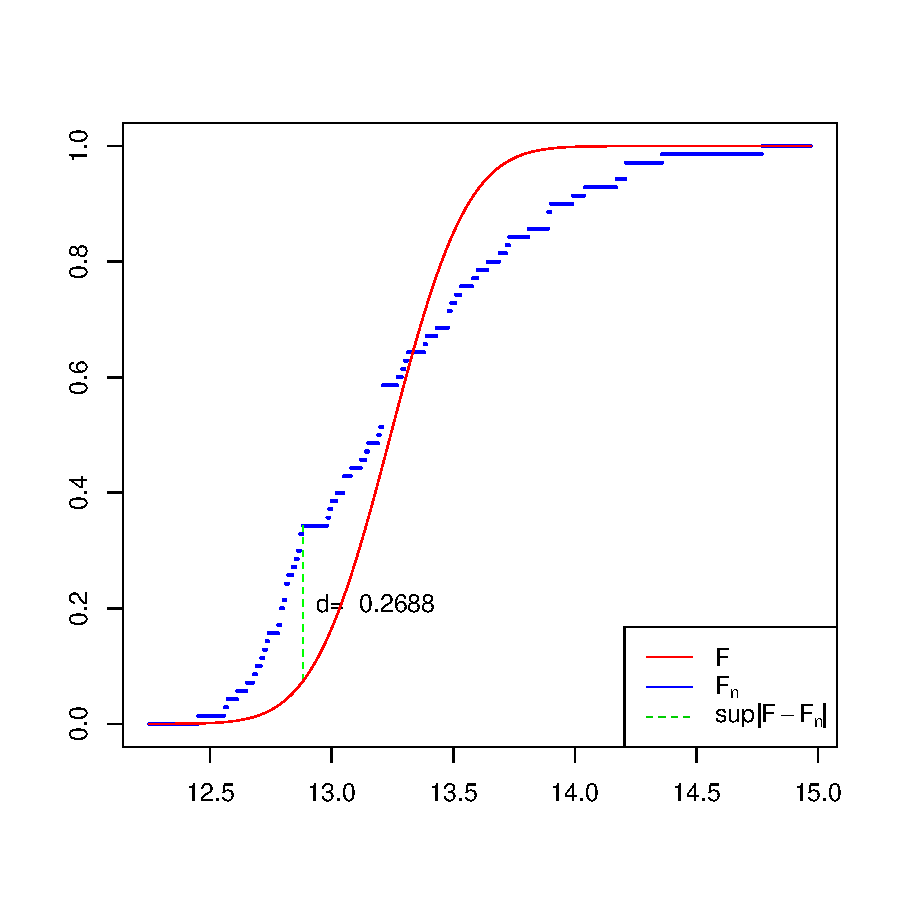
\includegraphics[width=\columnwidth]{Report-empiricTeorFunc}
	\end{figure}
\vspace{-1.5cm}
\begin{center}
Glass Type 1, Sodium (Na)
\end{center}}
\end{columns}

\vspace{15cm}
}

\begin{frame}[fragile]
\frametitle{Kolmogorov-Smirnov Test}
\framesubtitle{Improvement}
KS test is improved by solving the following
optimization problem \[KS(\mu,\sigma^2)=\sup_{x \in
\mathbb{R}}|F_n(x)-F(x,\mu,\sigma^2)|\to \min.\]
\begin{itemize}
\item<1->[]$R$ code used:
\item<2->[]
\begin{Schunk}
\begin{Sinput}
 c(mean(dat),var(dat))
\end{Sinput}
\begin{Soutput}
[1] 13.2422857  0.2493019
\end{Soutput}
\begin{Sinput}
 #optim is a predifined R function in stats package
 #defalut method of optimization is Nelder and Mead
 result = optim(c(mean(dat),var(dat)),KS)
 result$par
\end{Sinput}
\begin{Soutput}
[1] 13.1769501  0.4682486
\end{Soutput}
\begin{Sinput}
 result$value
\end{Sinput}
\begin{Soutput}
[1] 0.07870673
\end{Soutput}
\end{Schunk}
\end{itemize}
\vspace{10cm}
\end{frame}


\frame{
\frametitle{Kolmogorov-Smirnov Test}
\framesubtitle{Improvement}
KS test is improved by solving the following
optimization problem \[KS(\mu,\sigma^2)=\sup_{x \in
\mathbb{R}}|F_n(x)-F(x,\mu,\sigma^2)|\to \min.\]
\begin{columns}[t]
\column{0.5\columnwidth}
\vspace{-1cm}
\begin{itemize}
\item<1->Initial vector of parameters
$\mu=13.2423,\quad
\sigma^2=0.2493$
\item<1->Optimized vector of parameters
$\hat{\mu}=13.1770, \quad
\hat{\sigma}^2=0.4682$
\item<3->
$D_n=\sqrt{n}
\sup|F_n-F_{new}|=0.6585$
\item<4->
$c=1.6276$
\item<5->
$D_n<c \implies  H_0$ \alert{not rejected}

\item<6-> 
$\implies \mathbb{P}= \mathbb{P}_0$

\item<7-> \alert{$\implies$
 data normally distributed!}
\end{itemize}

\column{0.5\columnwidth}
  \vspace{-1.9cm}
    \only<1>{
    \begin{figure}
	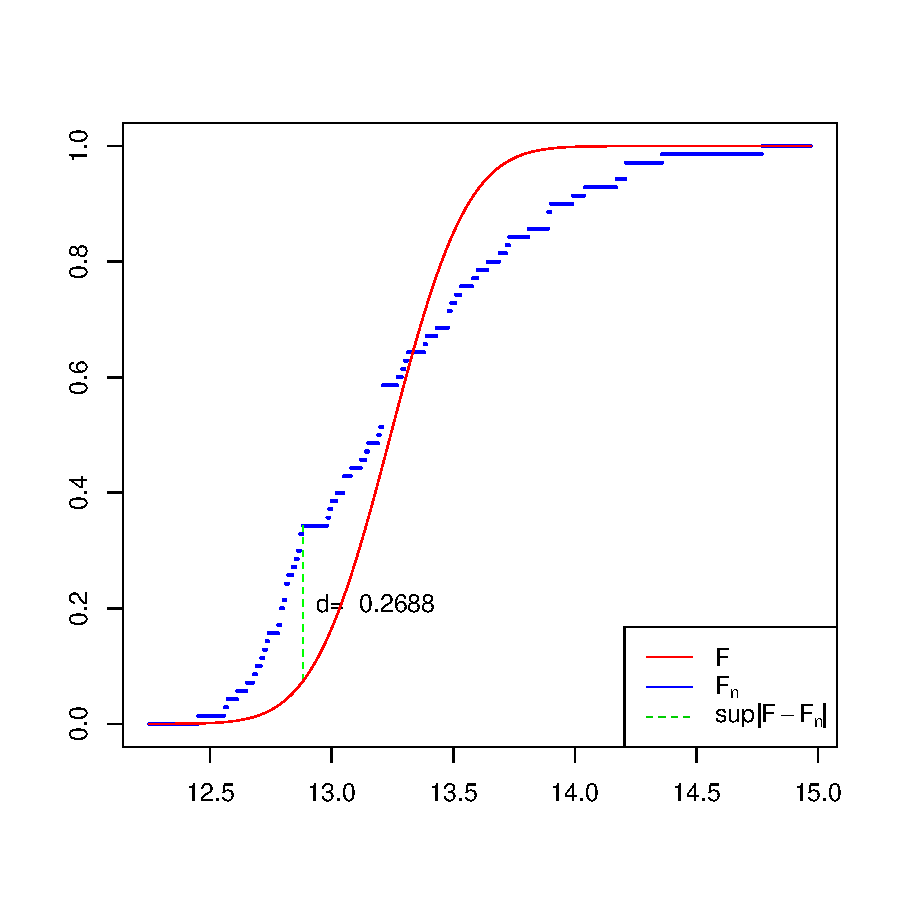
\includegraphics[width=\columnwidth]{Report-empiricTeorFunc}
	\end{figure}}
    \only<2->{
    \begin{figure}
	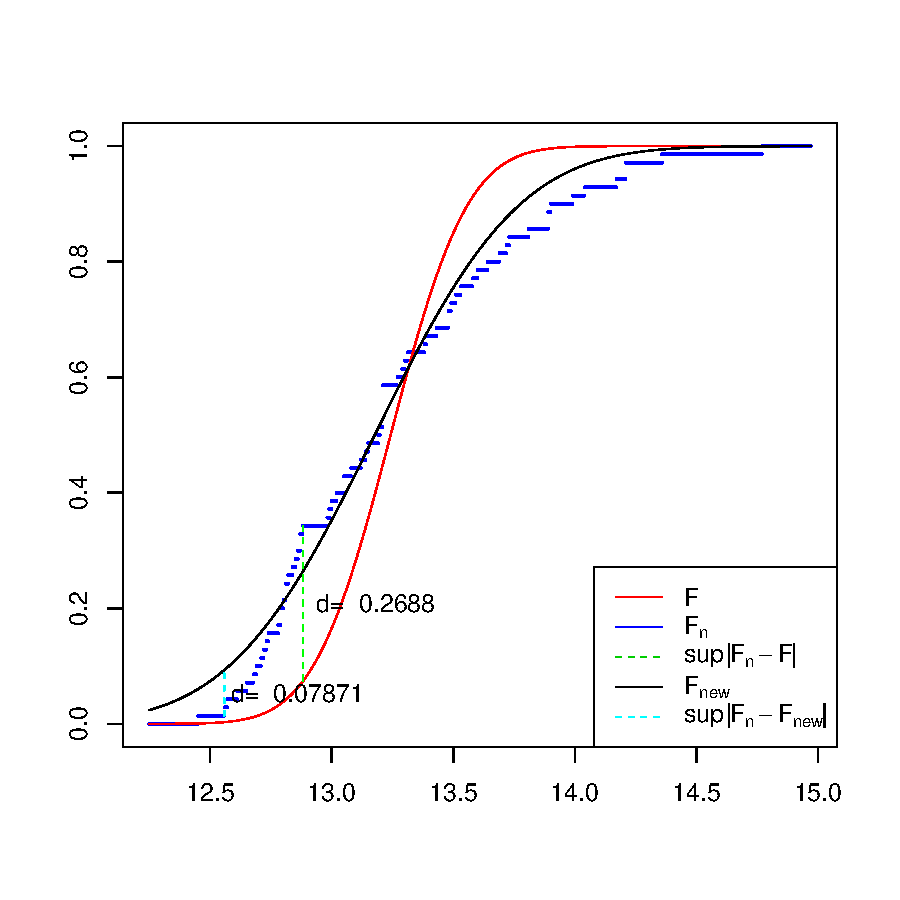
\includegraphics[width=\columnwidth]{Report-improvedKS}
	\end{figure}}
\onslide<2->{
\vspace{-1.5cm}
\begin{center}
Glass Type 1, Sodium (Na)
\end{center}}
\end{columns}

\vspace{15cm}
}


\frame{
\frametitle{Kolmogorov-Smirnov Test}
\framesubtitle{Results of the improved test on the whole data set}
\scriptsize
\begin{table}[h!]
\centering
\begin{tabular}{|cccccc|} \hline variable & test statistic & sig. level & critical value & p-value & rejected\\ \hline RI & 1.34 & 0.01 & 1.63 & 0.0561963016778131 & no\\ 
Na & 0.87 & 0.01 & 1.63 & 0.43825271603342 & no\\ 
Mg & 2.94 & 0.01 & 1.63 & 6.18457917100912e-08 & yes\\ 
Al & 0.84 & 0.01 & 1.63 & 0.474757887353829 & no\\ 
Si & 0.96 & 0.01 & 1.63 & 0.314710019077325 & no\\ 
K & 2.14 & 0.01 & 1.63 & 0.000212776619708754 & yes\\ 
Ca & 1.33 & 0.01 & 1.63 & 0.057710602872685 & no\\ 
Ba & 2.60 & 0.01 & 1.63 & 2.75476085742632e-06 & yes\\ 
Fe & 4.68 & 0.01 & 1.63 & < 1.0e-15 & yes\\ \hline \end{tabular}
\end{table}
}

\frame{
\frametitle{Kolmogorov-Smirnov Test}
\begin{columns}[t]
\column{0.3\columnwidth}

{\bf \centerline{Test Results:}}
\begin{table}[h!]
\centering
\begin{tabular}{|cc|} \hline variable & rejected\\ 
\hline 
RI & no\\ 
Na & no\\ 
Mg & yes\\ 
Al & no\\ 
Si & no\\ 
K & yes\\ 
Ca & no\\ 
Ba & yes\\ 
Fe & yes\\ 
\hline 
\end{tabular}
\end{table}

\column{0.7\columnwidth}
\only<2->{
\vspace{-1.35cm}
\begin{figure}
	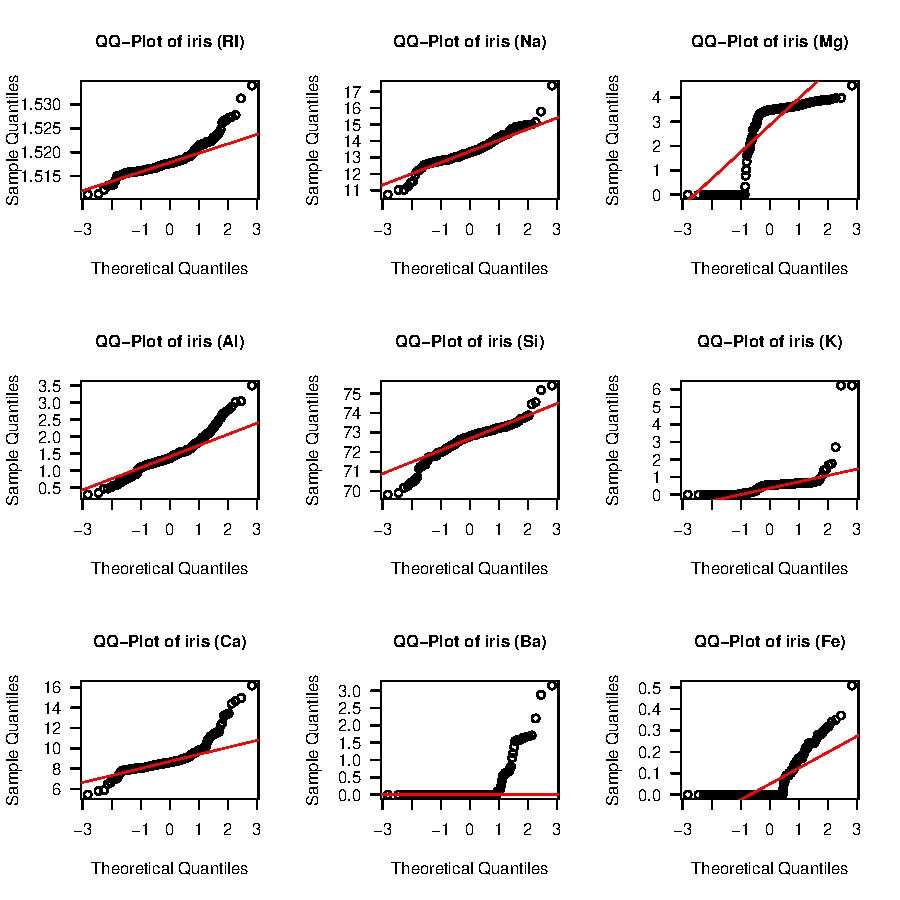
\includegraphics[width=\columnwidth]{auxiliary-drawQQPlots}
	\end{figure}}
\end{columns}
\vspace{15cm}
}

\frame{
\frametitle{Kolmogorov-Smirnov Test}
\framesubtitle{Results on the data subsets}
\scriptsize
\begin{table}[h!]
\centering
\vspace{-0.2cm}
\begin{tabular}{|cccccc|} \hline variable & test statistic & sig. level & critical value & p-value & rejected\\ \hline RI & 1.31 & 0.01 & 1.63 & 0.0630043926883292 & no\\ 
Na & 0.66 & 0.01 & 1.63 & 0.77871853343362 & no\\ 
Mg & 0.49 & 0.01 & 1.63 & 0.967729719418776 & no\\ 
Al & 0.92 & 0.01 & 1.63 & 0.366854549713195 & no\\ 
Si & 1.06 & 0.01 & 1.63 & 0.208027646546284 & no\\ 
K & 1.73 & 0.01 & 1.63 & 0.00491847745617136 & yes\\ 
Ca & 0.84 & 0.01 & 1.63 & 0.48064266616439 & no\\ 
Fe & 2.65 & 0.01 & 1.63 & 1.63244296669252e-06 & yes\\ \hline \end{tabular}
\caption{\scriptsize Test results of the improved KS test on type 1 glass}
\end{table}
\vspace{-0.5cm}
\begin{table}[h!]
\centering
\begin{tabular}{|cccccc|} \hline variable & test statistic & sig. level & critical value & p-value & rejected\\ \hline RI & 0.67 & 0.01 & 1.63 & 0.767837508224946 & no\\ 
Na & 0.52 & 0.01 & 1.63 & 0.951658259816235 & no\\ 
Al & 0.49 & 0.01 & 1.63 & 0.968495966845634 & no\\ 
Si & 0.56 & 0.01 & 1.63 & 0.915628110530136 & no\\ 
K & 1.43 & 0.01 & 1.63 & 0.0340401962712393 & no\\ 
Ca & 0.56 & 0.01 & 1.63 & 0.91558957374917 & no\\ 
Ba & 0.76 & 0.01 & 1.63 & 0.61288183743927 & no\\ \hline \end{tabular}
\caption{\scriptsize Test results of the improved KS test on type 7 glass}
\end{table}
}

\subsection{Multivariate case}

\frame{
\frametitle{Chi-Square Plot for Multivariate Normality}
\begin{block}{Sample mean and covariance matrix}
Multivariate sample $X=(X_1,X_2,\dots,X_n)$ with \alert{$p$} variables
$X=(X_1,X_2,\dots,X_n)$ $\bar{X}=\frac{1}{n}\left(\sum \limits_j X_j\right) \quad S=\frac{1}{n-1}\left(\sum \limits_j (X_j-\bar{X})(X_j-\bar{X})'\right)$
\end{block}
\begin{block}{Generalized squared distances}
$d^2_j= (X_j-\bar{X})'S(X_j-\bar{X})', \quad j=1,2,\dots n$\\
\[\alert{d^2_j\approx \chi^2_p}\]
$d^2_{(1)}\le d^2_{(2)} \le \dots \le d^2_{(n)}$ - empirical quantiles\\
$q_{(j)} = (\chi^2_p)^{-1}\left(\frac{j - \frac{1}{2}} {n}\right)$ - theoretical quantiles\\
\alert{$\implies$}  Plot $d^2_{(i)}$ against $q_{(i)}$
\end{block}
\vspace{15cm}
}

\frame{
\frametitle{Chi-Square Plot for Multivariate Normality}
\vspace{-1cm}
\begin{columns}[t]
\column{0.5\columnwidth}
\begin{figure}
	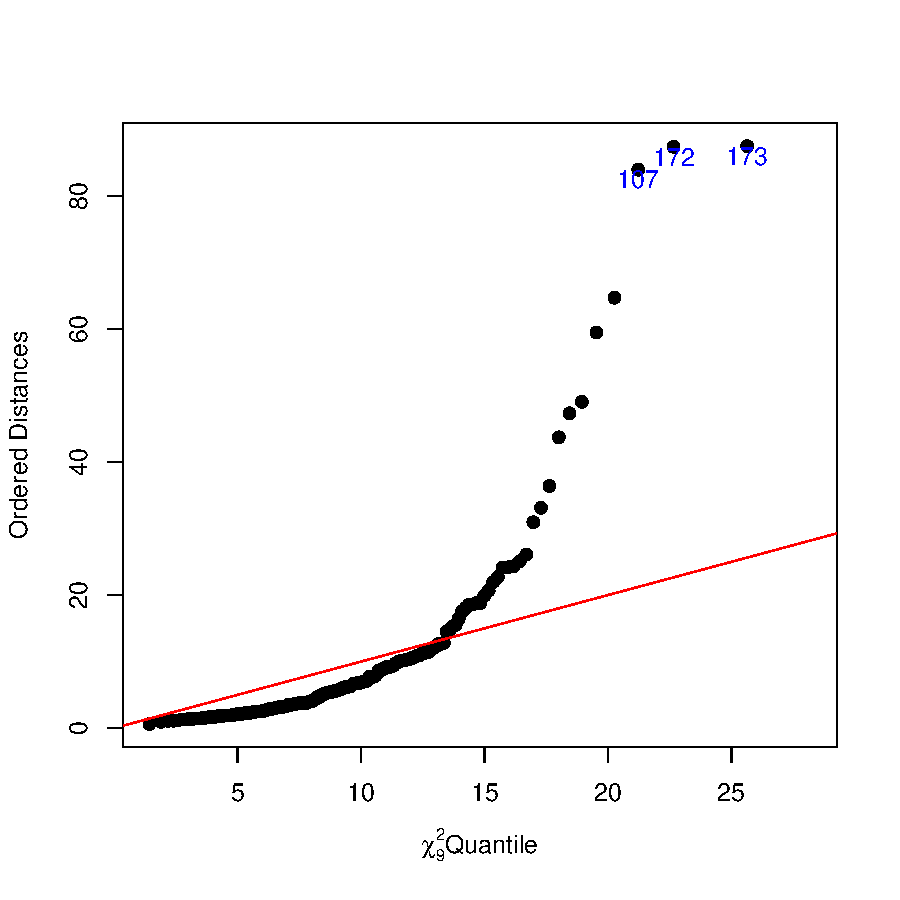
\includegraphics[width=\columnwidth]{auxiliary-drawChiSquarePlotFull}
    \caption{The whole data set}
\end{figure}
\column{0.5\columnwidth}
\begin{figure}
	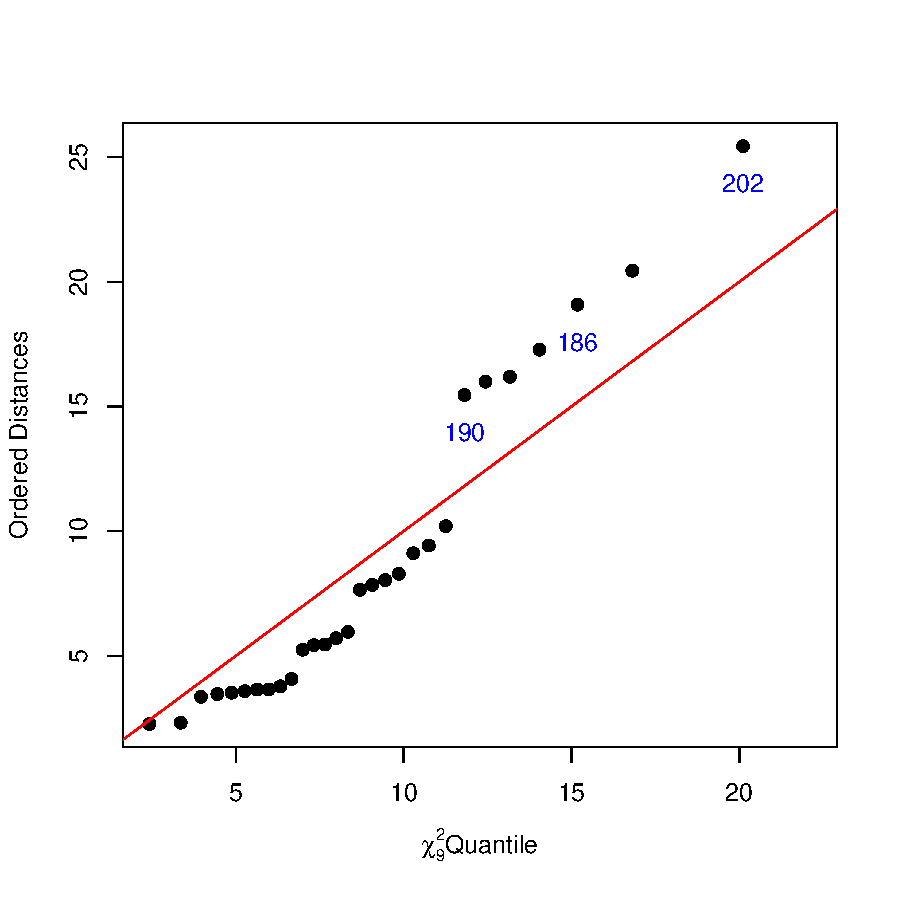
\includegraphics[width=\columnwidth]{auxiliary-drawChiSquarePlotType7}
    \caption{Type 7 Glass}
\end{figure}
\end{columns}
}


\frame{
\frametitle{Plot of multivariate normal distribution}
\framesubtitle{Theoretical foundations}
\bi
\item Contour lines of the plot of a multivariate normal distribution are shaped \hl{elliptically}
\item Ellipsoids are centered at $\mu : \left\{x:(x-\mu)'\, \Sigma^{-1}(x-\mu) = c^2\right\}$ with some constant $c$.
\ei

\begin{example}
\small
\begin{minipage}{0.50\textwidth}
Multivariate normal distribution with sample size 500 and parameters

\begin{displaymath}
  \begin{array}{rcl}
                 \mu & = & \left(\begin{array}{c} 1\\ 2\end{array} \right)\\
                 \phantom{.} & \phantom{.} & \phantom{.}\\
                 \Sigma & = & \left[\begin{array}{cc} 27 & 15\\ 15 & 18\end{array} \right]
  \end{array} 
\end{displaymath}


%\[\mu = \left(\begin{array}{c} 1\\ 2\end{array} \right), \quad \Sigma = \left[\begin{array}{cc} 27 & 15\\ 15 & 18\end{array} \right]\]
\end{minipage}
\hfill
\begin{minipage}{0.4\textwidth}
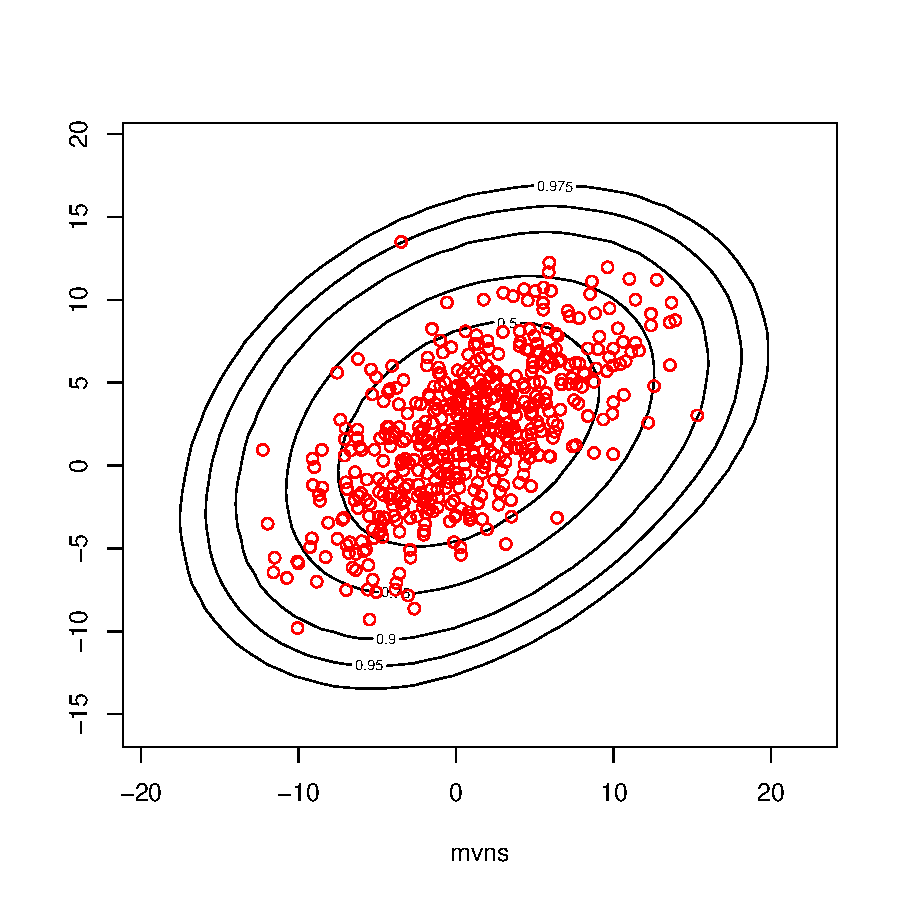
\includegraphics[width=0.8\textwidth]{report-plotMVNSim}
\end{minipage}
\end{example}
}

\frame{
\frametitle{Plot of multivariate normal distribution}
\framesubtitle{Application}
\bi
\item Concerning the complete sample, the p-values for the variables Na and Al are highest among all used test methods.
\item Plot data points and determine contour lines.
\ei
\begin{center}
\only<1>{\includegraphics[width=0.5\textwidth]{report-contourGlassNaAl}}
\only<2>{\includegraphics[width=0.5\textwidth]{report-cluster7}}
\only<3>{\includegraphics[width=0.5\textwidth]{report-contourGlassNaAl-7}}
\end{center}
}

\section{Summary}

\frame{
\frametitle{Summary}
\bi
\item Normal distribution is assumed for many statistical methods.
\item Test methods for normality
  \bi
  \item Q-Q-plot
  \item Shapiro-Wilk test
  \item Chi-squared test
  \item Kolmogorov-Smirnov test
  \item Plotting contour lines for the multivariate case
  \item Chi-squared plot
  \ei
\item The tests return different results but often have similar tendencies.
\item Box-Cox transformation is only suited for unimodal and not too noisy data.
\item Data from the \texttt{Glass}-package appear to be heterogenuous in the complete sample but rather not for specific types.
\ei
}

\appendix
\againframe<2>[noframenumbering]{zoom}

\end{document}
